

In this section I will examine the robustness of the results by altering the model variables or event requirements and re-estimate the results, as it is important to cross-validate that a potential appearance of over-performance is not created artificially. Thus, the practice can lead to validation or invalidation along with advancement of model specifications. 

\subsection{Market model: event specification} \label{sec: sens_st_sd}
The requirement rule for event identification is based on the magnitude of events in relation to the average event for the individual firm. Thus, it seems plausible that an increase in the tightness of the requirement rule will lead to higher abnormal returns in absolute values.  
To address the issue I test whether the short term abnormal returns are sensitive to the methodology in specifying individual events. Specifically, I re-estimate the models with a requirement stating that the events should be more than, respectively, two and three standard deviations from the average event. A tighter event specification determine that fewer stocks will be included in the model as less events will be regarded as important. Consequently, the events included should be more negative or positive with a stricter rule. 



The results are reported in table \ref{tab: ST_significace}, which demonstrate that negative events continue to generate significant abnormal returns, while positive events does not. Due to insignificance and borderline randomness of the relation between positive events and returns I will only present the plots related to negative events. The graph of the positive events can be found in Appendix \ref{fig:ST_pos_sensi}. 


\begin{figure} [h]
    \centering
    \caption{Negative news: Update event requirement}
    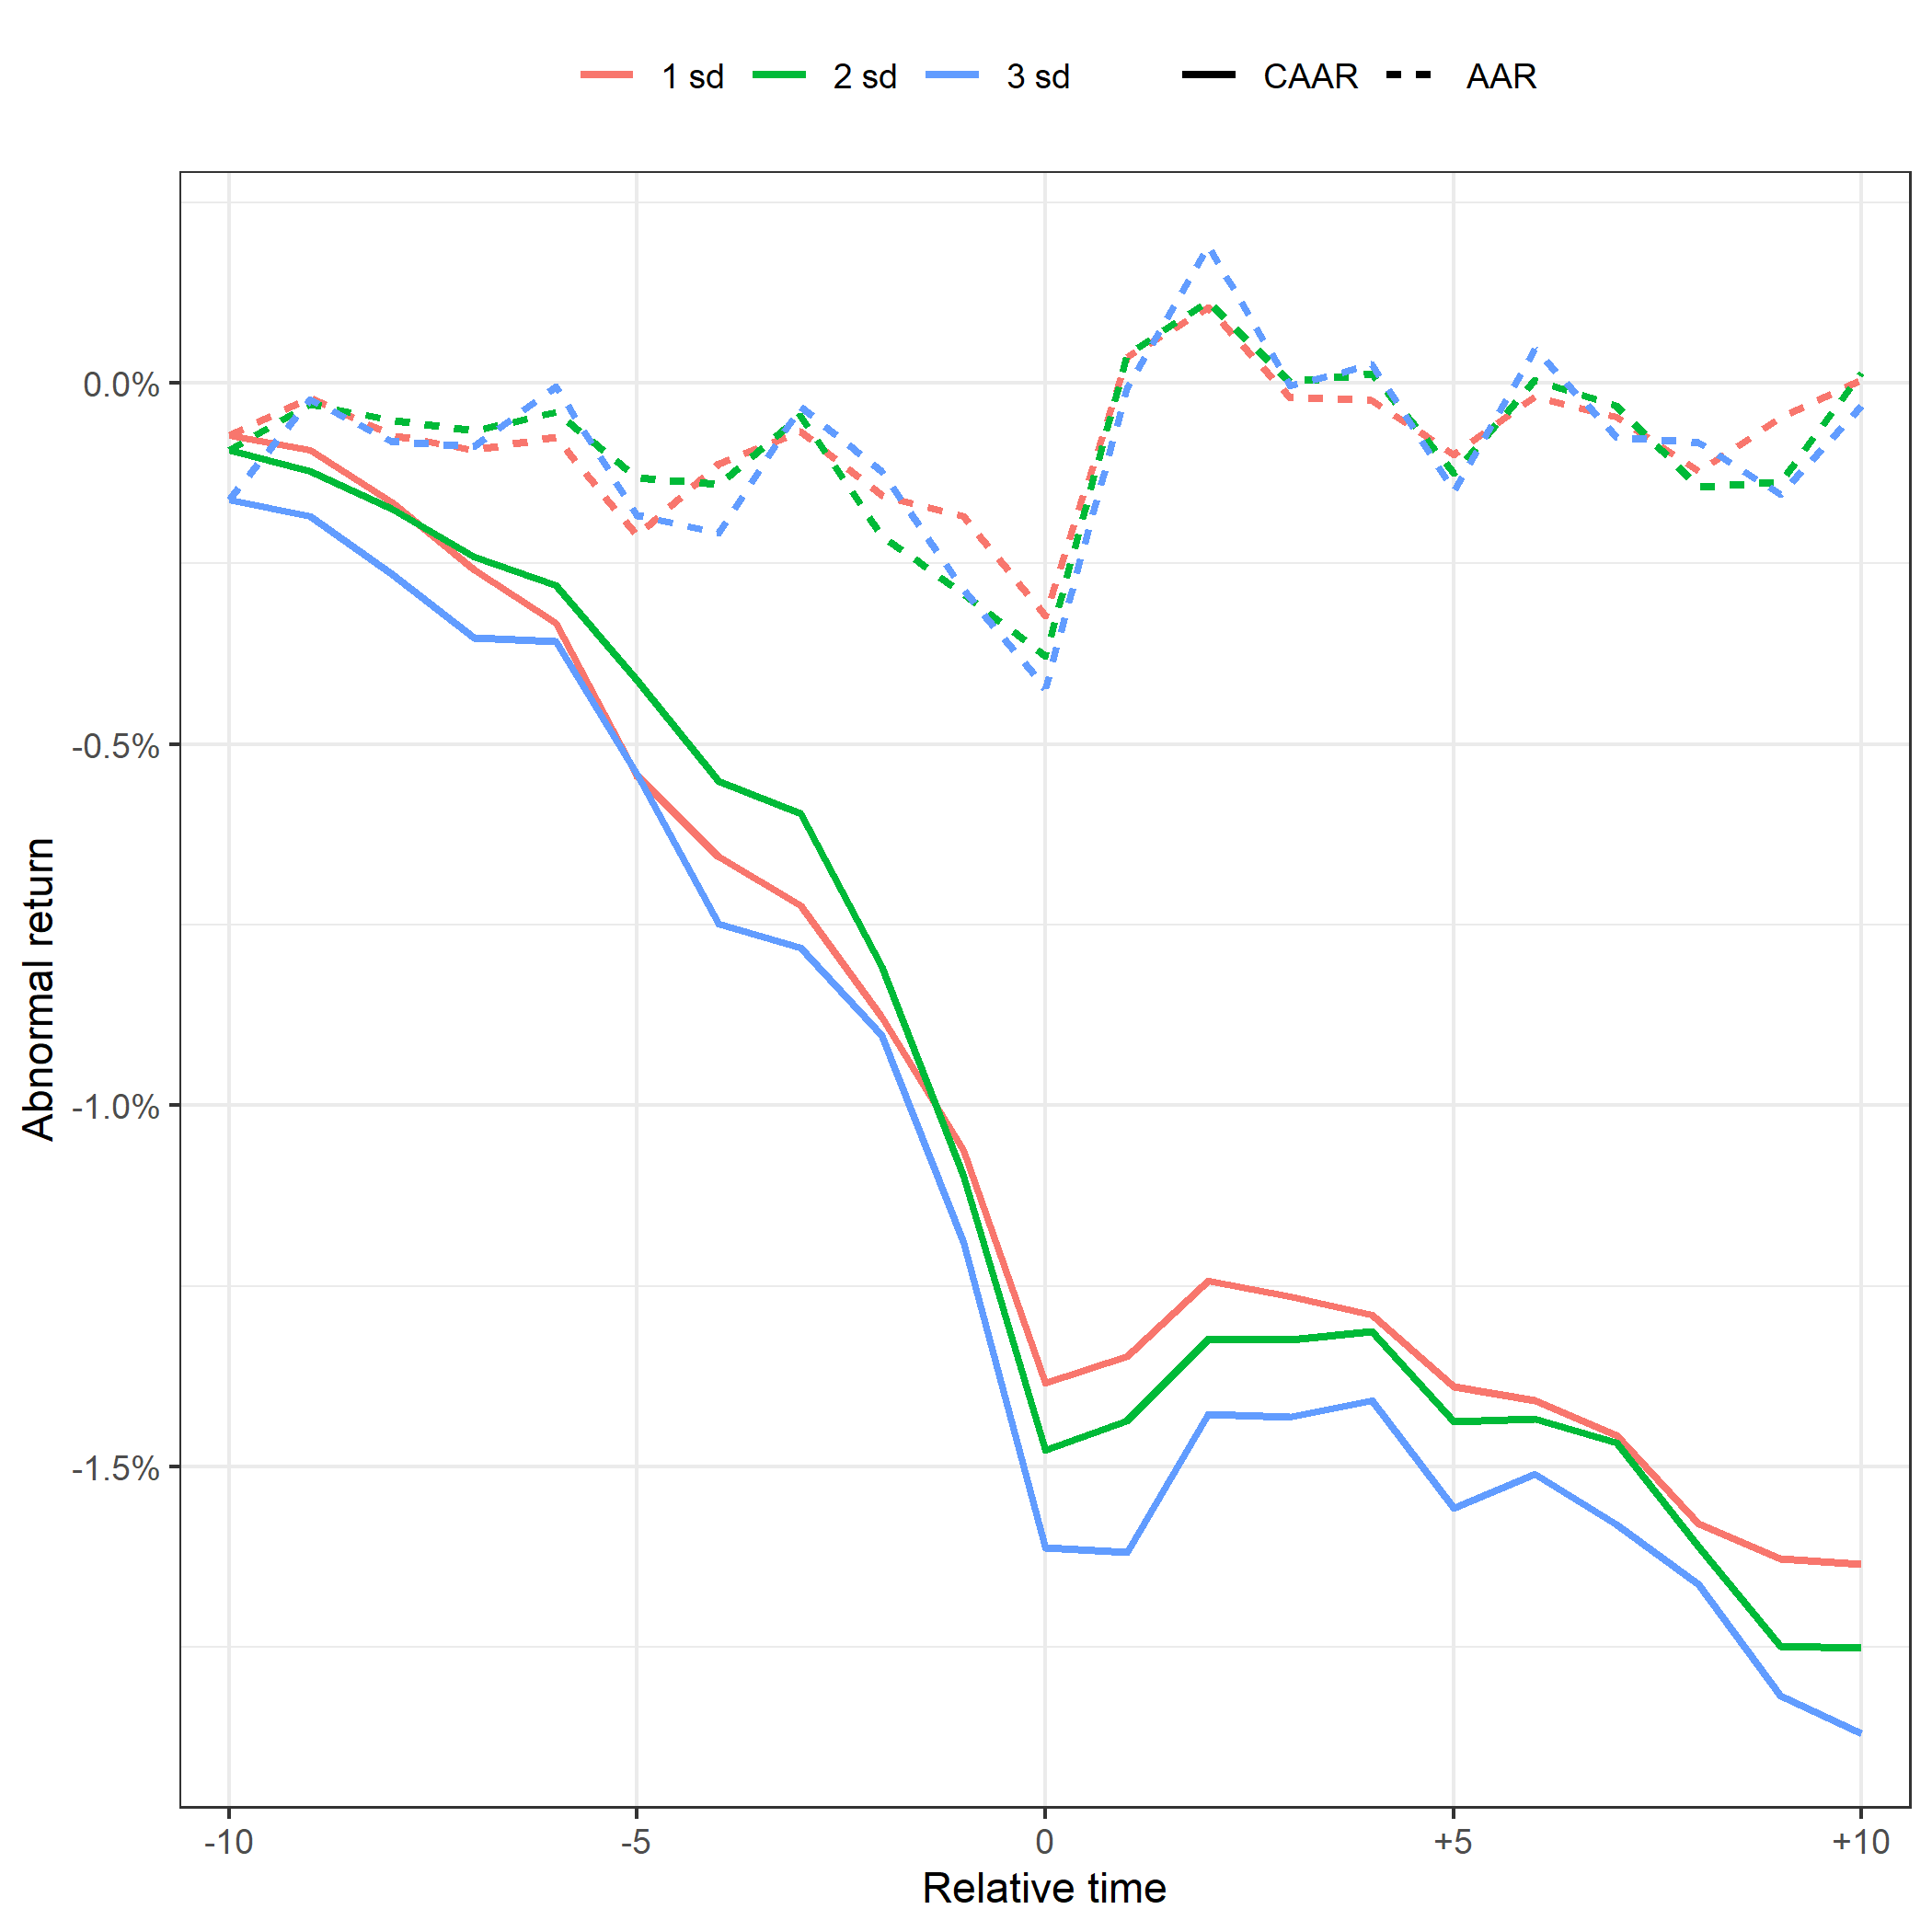
\includegraphics[scale=0.6]{Projekt/1.Figures analysis/ST_negative_sensitivity.png}
     \caption*{\footnotesize The figure illustrates the average abnormal return (AAR) and cumulative AAR (CAAR) around the event date (t = 0) of negative news. The various colors represent whether the event identification rule was based on 1, 2, or 3 standard errors.  }
    \label{fig:ST_neg_sensitivity}
\end{figure} 

The two new models based on negative events are compared to the original results (1 sd) in figure \ref{fig:ST_neg_sensitivity}. The AAR is presented in dotted lines and the CAAR in solid lines along with estimation requirements of 1 sd (red), 2 sd (green), and 3 sd (blue). For simplicity, I have skipped the confidence intervals along with the barchart, which represented the relative amount of events. The similarities of the AAR and CAAR imply that the results are robust to changes in the event specification. While it is clear that enforcing a stronger sd requirement leads to lower AARs on the event date, no effect on the CAAR is present, visually, over the full event window. From table \ref{tab:ST_sensitivity}, the AAR on $t=0$ is, respectively, -0.52\% and -0.61\% for the 2 and 3 sd requirements compared to -0.37\% for the original 1 sd, meaning that the greatest instantaneous causal impact happens with a tight event rule. All are significant on the 1\% level. Intuitively, the investor reaction is more severe when events are identified as more important.  



\subsection{Market model: value vs. equal weights} \label{sec: sens_st_weights}

A portfolio of stocks needs to be weighted in order to determine the relative impact the individual constituents have on the performance of the portfolio. Throughout the paper the portfolio weights have been based on the relative market capitalization of the firms - also known as value weights. Table \ref{tab:ST_sensitivity_weights} compares the performance of the value weighted portfolio against an equal weighted. The portfolios hold the same firms, however with different weights, and are based on the same identified events. Again, the results from using equal weights show that none of the portfolio returns, associated with positive events, are significant. 

\begin{figure}[H]
    \centering
    \caption{Negative news: Value vs. Equal weights}
    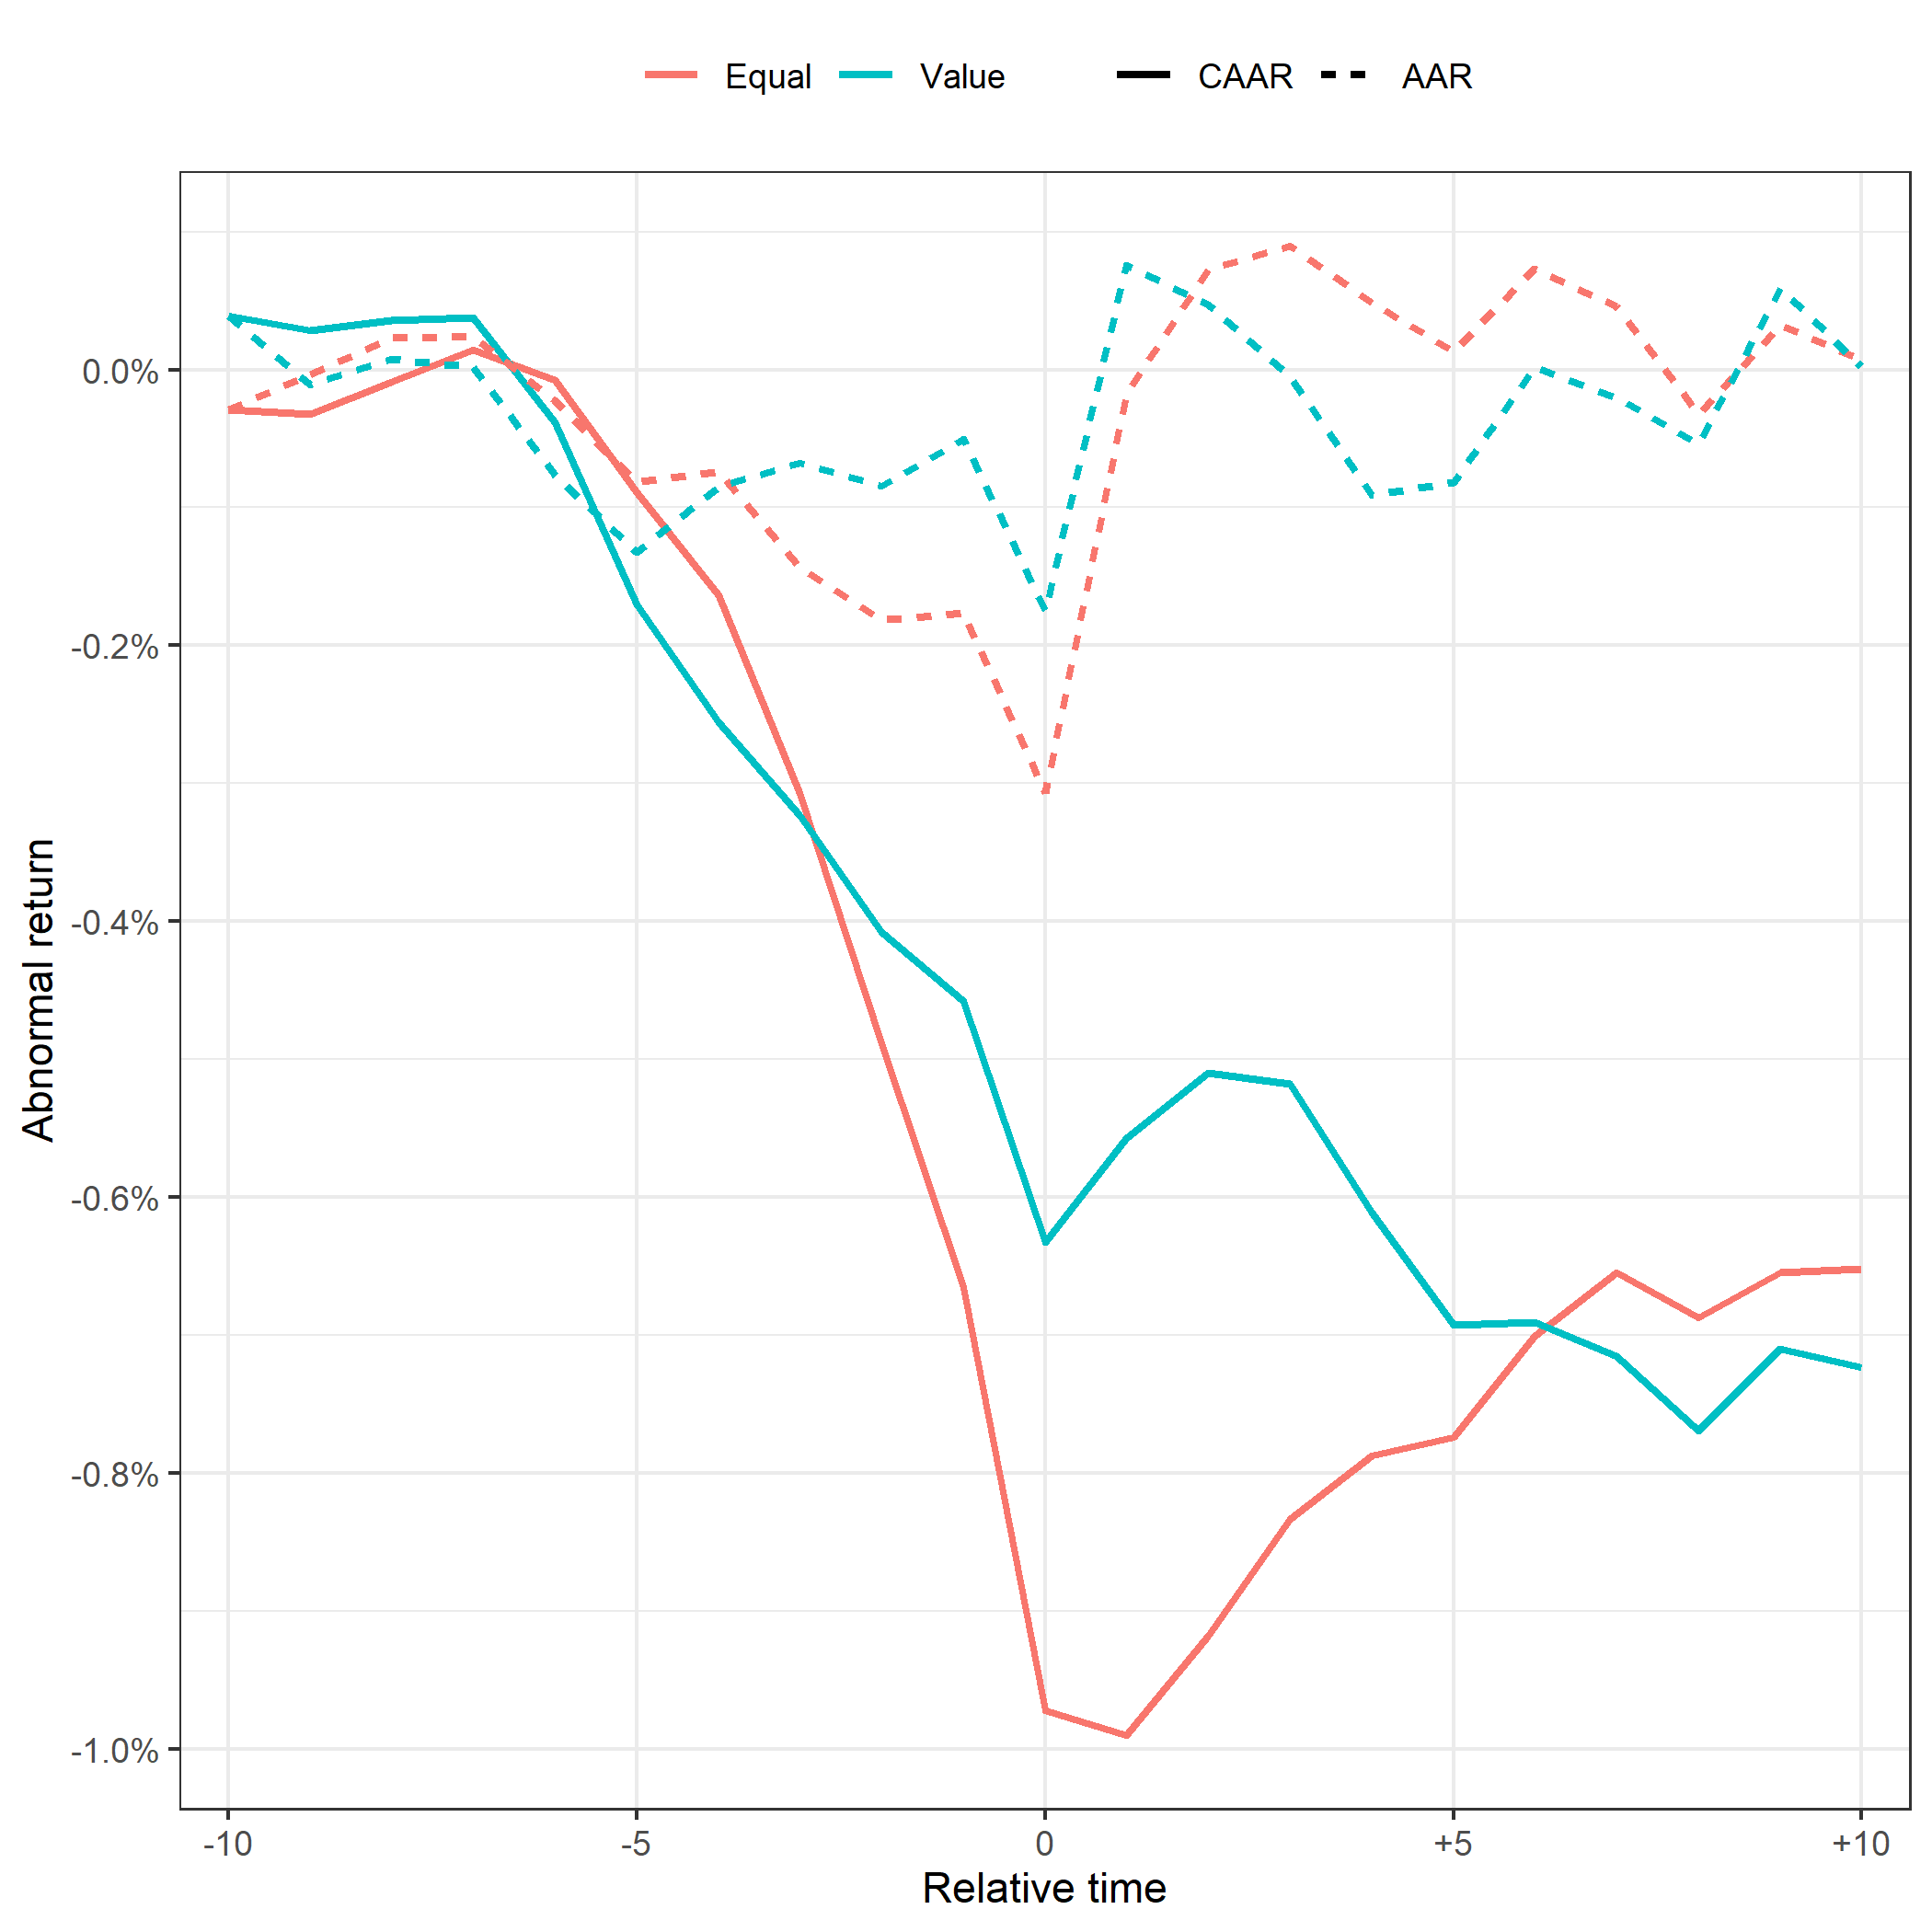
\includegraphics[scale=0.6]{Projekt/1.Figures analysis/ST_negative_sensitivity_weight.png}
     \caption*{\footnotesize The figure illustrates the average abnormal return (AAR) and cumulative AAR (CAAR) around the event date (t = 0) of negative news. The blue lines are returns calculated from an equally weighted portfolio, while the red lines are based on market capitalization weights.}
    \label{fig:ST_neg_sensitivity_weight}
\end{figure} 


The equal weighted portfolio returns associated with negative events the empirical results from the former section is more or less valid. As expected, the returns are slightly different. However, they do appear significant on the same level and with the same direction of returns as the original results. While the portfolio AARs apparently follow each other to some extent, the development in CAAR is more adverse using equal weights relative to value weights. A potential explanation is that an equal weighted portfolio will award more weight to small stocks, thus they will contribute more to the portfolio returns relative to an value weighted portfolio. As small stocks tends to be more volatile than larger stocks \cite{Fama_french_3fac}, negative news could drive portfolio returns lower. 



In the period following a given event, the average reaction from equal and value weighted portfolios are different. Although the AARs at this point are insignificant, the CAAR series indicate that the equal weighted portfolio, which favor small stocks, is pricing in events in the days following an actual event, whereas most of the negative price action is happening before the event has occurred for the value weighted portfolio. Possibly, news about small stocks will take time to reach a large amount of investors, which is why the price reaction is happening at a later point. 




\subsection{Calendar Time Portfolio: Portfolio weights}

The sensitivity of returns in relation to the weights used in calculating portfolio returns will also be controlled in regards to the long term abnormal returns. Since the returns associated with positive events were insignificant in the initial analysis, this section will exclusively report on the results relating to negative events. 

Table \ref{tab: FF5_neg_sensi_weights} reports the alphas, t-values and significance levels of equally weighted portfolios. Besides the weights, the portfolio construction is identical to that from the empirical results in section \ref{sec: long_term_portfolio}. The results clearly indicate a discrepancy between value and equal weights with the latter generating higher absolute alpha values. For example, the value weighted portfolio with SD = 2 and T = 1 generated an insignificant alpha of -0.47, while the equivalent equal weighted portfolio generated an alpha of -0.94 significant on the $1\%$ level.   

The results are in accordance with the short term sensitivity analysis on portfolio weights, where the equal weighted Market Model portfolio generated lower abnormal returns as well. As before, a potential explanation for the severity of the alphas are due to smaller stocks receiving a higher relative weight in the equal weighted portfolio. In accordance, the regression summaries report that the portfolio with SD = 1 and T = 1 is highly sensitive towards the size factor with a beta-value of 0.97. However, the negative returns of the constructed portfolios are more severe than explainable by the SMB factor, which gives rise to the alpha generation. A look-back periods of T = 8 and 12 months generate significant alpha as well,  Smaller stocks seems to be punished harder for negative news than larger stocks. However, this is not the focus of the paper. The returns of the equal weighted portfolios confirm the negative association between negative events and abnormal returns and to some degree the magnitude of the value weighted portfolio returns.


\subsection{Calendar Time Portfolio: Excess return}

An inherent assumption of the factor model is that investors can borrow and lend at the risk-free rate. This is not a practical assumption. Hence, the returns of the models can be sensitive to the assumption of the market return. 
To review the impact of the risk-free rate on abnormal returns, I re-estimate the models with the assumption that the rate is zero. This step applies to both sides of the equation in \ref{eq: FF5}, where $R_{rf,t}$ is set to zero. 

The alphas, t-values and significance levels for the portfolios with the risk-free rate assumed to be zero are reported in table \ref{tab: FF5_neg_sensi_rf}. Generally, the r-squared of the regressions are relatively high with values between 0.82 and 0.98. 

The factor models are not very sensitive to changes in the market index and the risk-free rate, as the alphas are close to or slightly more negative than the original values.  With interest rates close to zero in this period, this result may not be overly surprising. Nonetheless, the adjustment does ensure that the portfolio alpha with SD = 3 and T = 1 becomes significant at the $10\%$ level. Setting the rate to zero essentially increases the portfolio returns (response variable) and the market returns (explanatory variable) as the rate was originally subtracted from these. Intuitively, a higher alpha would be expected as the excess returns increases. However, the reduced alpha originates from a slightly increased sensitivity towards the size and value factors and less sensitivity to the market portfolio.       


\setlength{\tabcolsep}{15pt}
\begin{table}[h]
\small
\centering
\caption{FF-5 alpha with equal weights and edit event rule } 
\makebox[\textwidth][c] {
\begin{tabular}{ccccccc}
\hline \hline \\ 
& &  Equal & & \multicolumn{2}{c}{ Value  } & \\ \cline{3-3} \cline{5-6}
  & & (1 SD) & & 2 SD  &  3 SD  & \\   
 & & & T = 1  & & \\ \cline{2-6}
 &  Alpha & $-0.96^{***}$  & &  -0.47  & -0.78  &  \\ 
 & t-value &  -3.94 &  & -1.33  & -1.63 & \\
 & &   & T = 4  & \\ \cline{2-6}
 & Alpha & $-0.70^{***}$ &  & $-0.45^{**}$ &  -0.27 & \\
 & t-value & -3.95 & & -2.12  & -1.04  & \\
 & &  & T = 8  & \\ \cline{2-6}
 & Alpha  & $-0.64^{***}$ & & -0.14 & -0.12 &  \\
 & t-value  & -4.20 & & -0.89 & -0.68 & \\
& &  & T = 12  & \\ \cline{2-6}
 & Alpha  & $-0.49^{***}$ &  & -0.16 & -0.17 &  \\
 & t-value & -3.71 & & -1.16 &  -0.97  & \\ \hline \hline
 \multicolumn{7}{l}{ \footnotesize $^* \; p\; <\; 0.1$, $ ^{**} \; p\; <\; 0.05$, $ ^{***} \; p\; <\; 0.01$  } \\
 \multicolumn{7}{p{12cm}}{ \footnotesize Alpha is the WLS-regression intercept (in \%) of the Fama-French 5-factor model, displayed along with the corresponding t-value. N is the average amount of firms included in the portfolio each month, and T is the portfolio holding period. The threshold for event firms to be included in the portfolio is either 1,2 or 3 "SD" (standard deviations) larger than the mean.} \\ 
 \hline
\end{tabular}
}
\label{tab: FF5_sensitivity}
\end{table}
